\chapter{Détection d'Anomalies par Machine Learning}

\section{Pipeline de traitement des données}

Le pipeline de Machine Learning a pour objectif de détecter automatiquement les comportements anormaux dans les flux de communication IoT. Le diagramme d'activité de la figure~\ref{fig:ml_pipeline} illustre l'ensemble du processus, depuis le chargement du dataset jusqu'à la comparaison des modèles.

\begin{figure}[H]
  \centering
  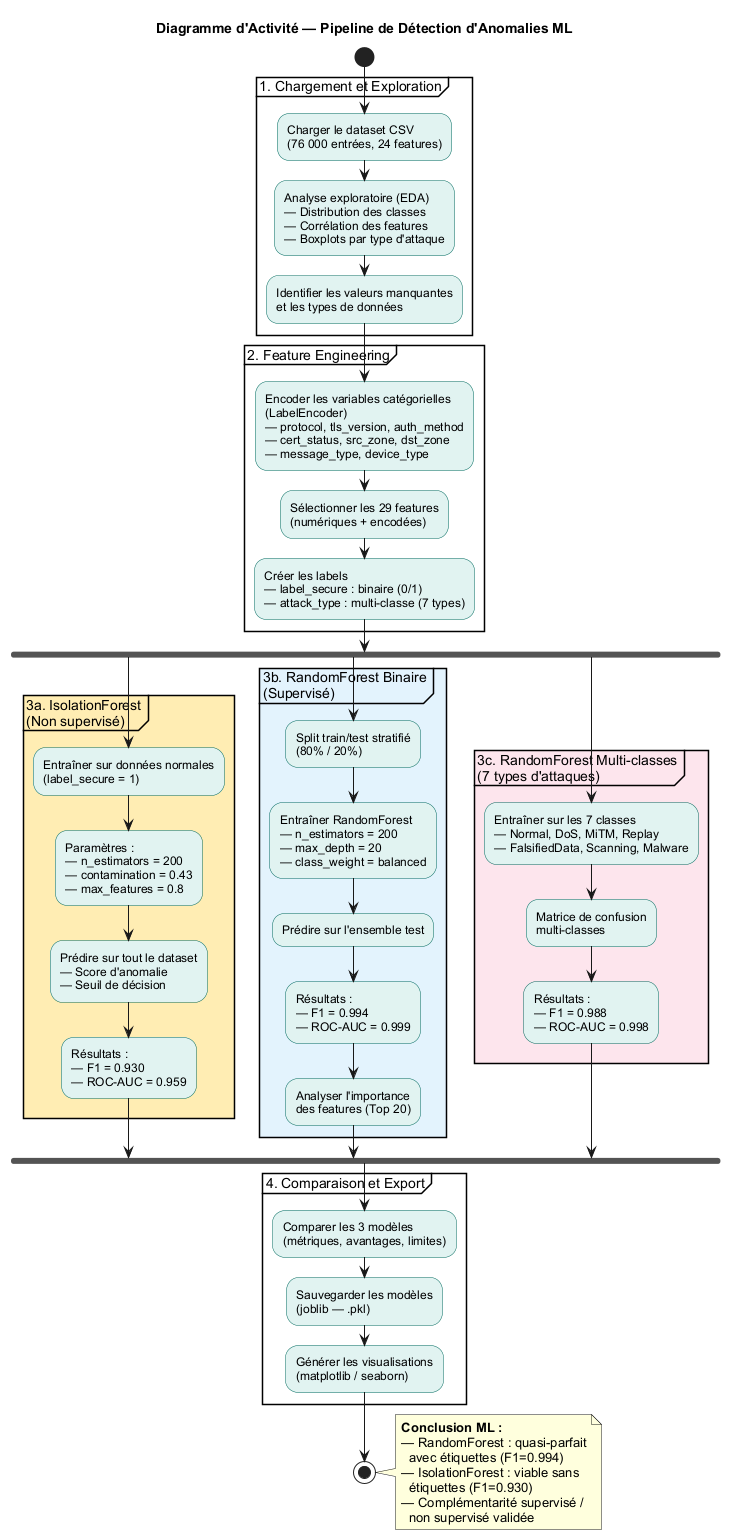
\includegraphics[width=0.65\textwidth]{diagrams/diag-ml-pipeline.png}
  \caption{Pipeline de détection d'anomalies par ML -- diagramme d'activité}
  \label{fig:ml_pipeline}
\end{figure}

\subsection{Chargement et exploration}

Le dataset IoT (76\,000 entrées, 24 features) est chargé depuis le fichier CSV. Une exploration descriptive préalable a permis d'identifier les caractéristiques statistiques de chaque classe.

\begin{figure}[H]
  \centering
  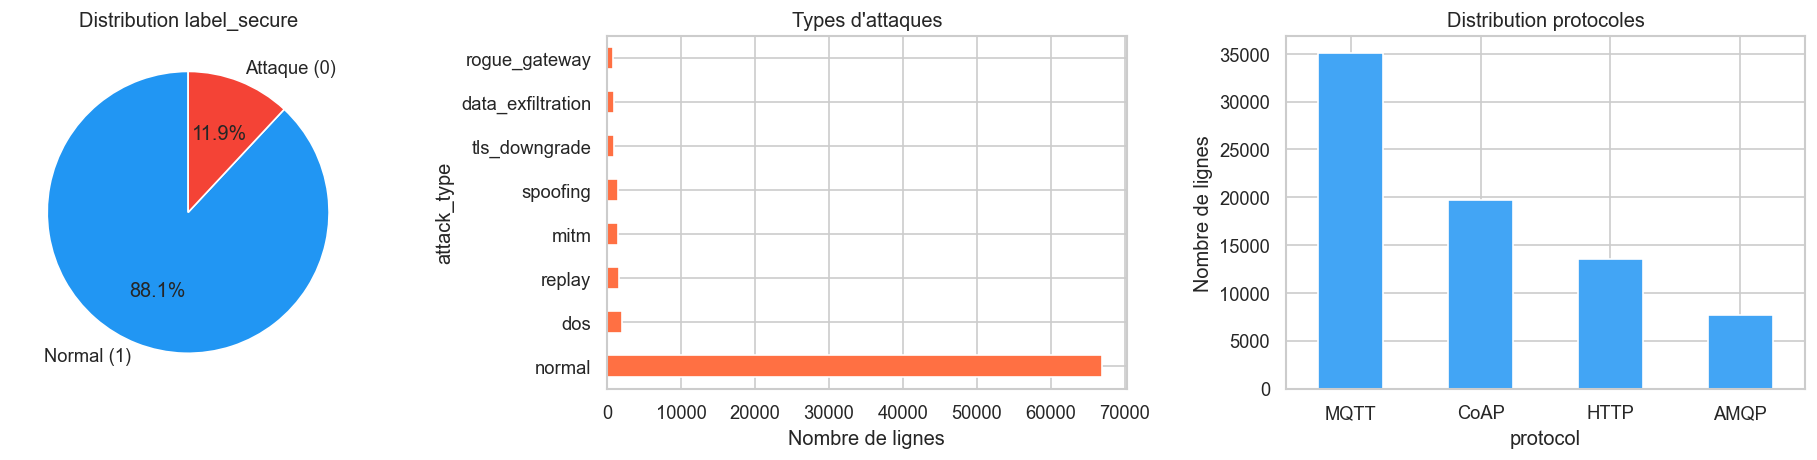
\includegraphics[width=0.8\textwidth]{figures/eda_classes_distribution.png}
  \caption{Distribution des classes dans le dataset (EDA)}
  \label{fig:eda_classes}
\end{figure}

\begin{figure}[H]
  \centering
  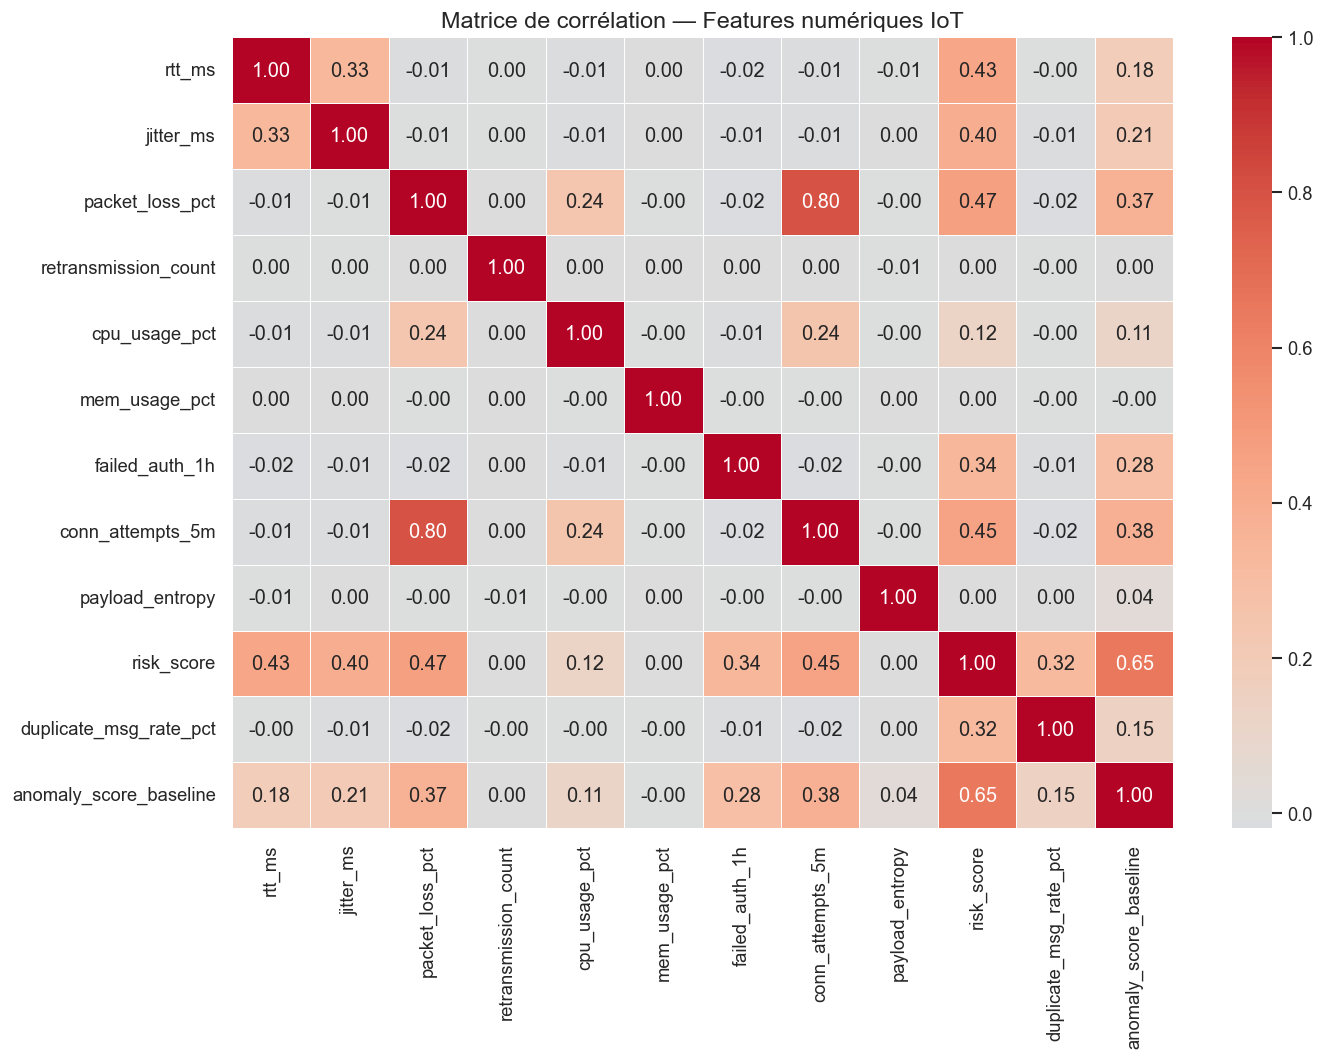
\includegraphics[width=\textwidth]{figures/eda_correlation_heatmap.png}
  \caption{Matrice de corrélation des features}
  \label{fig:eda_corr}
\end{figure}

\begin{figure}[H]
  \centering
  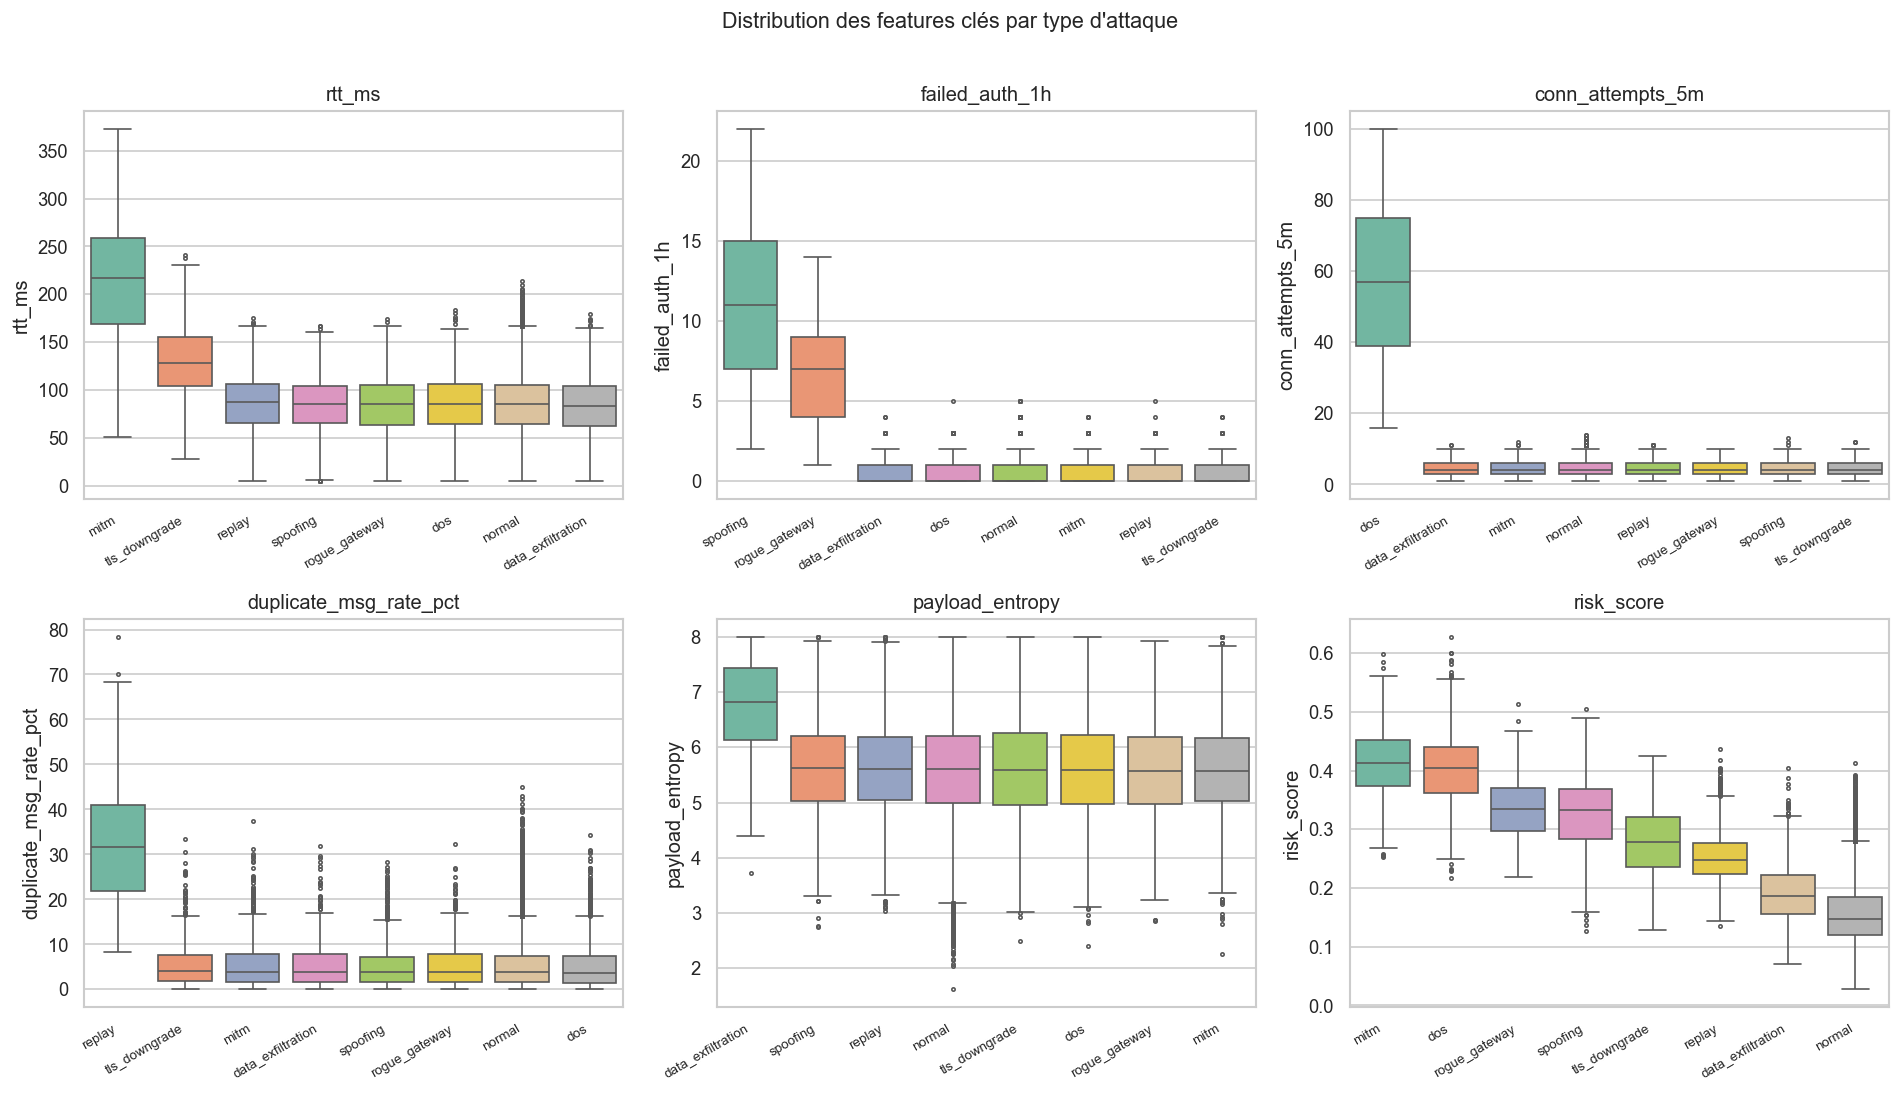
\includegraphics[width=0.9\textwidth]{figures/eda_boxplots_by_attack.png}
  \caption{Boxplots des features par type d'attaque}
  \label{fig:eda_boxplots}
\end{figure}

\subsection{Prétraitement}

Le prétraitement des données suit les étapes suivantes :
\begin{enumerate}
  \item \textbf{Encodage des variables catégorielles} : Les types d'attaques sont encodés numériquement via un \texttt{LabelEncoder}. Un label binaire (normal/anormal) est également créé.
  \item \textbf{Sélection des features} : Les colonnes d'identification (timestamps, flow IDs) sont exclues. Seules les features numériques pertinentes sont retenues.
  \item \textbf{Normalisation} : Un \texttt{StandardScaler} (centrage-réduction) est appliqué pour homogénéiser les échelles des features.
  \item \textbf{Split train/test} : Le dataset est divisé en 80\,\% / 20\,\% avec stratification pour maintenir les proportions de classes~\cite{scikit_learn}.
\end{enumerate}

Le code complet du pipeline de prétraitement est fourni en Annexe~A.

\section{Isolation Forest -- Détection non supervisée}

\subsection{Principe et configuration}

L'IsolationForest~\cite{liu2008isolation} isole les anomalies en construisant des arbres binaires aléatoires. Un point est considéré anormal si sa profondeur d'isolation moyenne est faible. Les hyperparamètres retenus sont :

\begin{table}[H]
\centering
\caption{Hyperparamètres de l'IsolationForest}
\label{tab:iso_params}
\begin{tabular}{ll}
\toprule
\textbf{Paramètre} & \textbf{Valeur} \\
\midrule
\texttt{n\_estimators} & 200 \\
\texttt{contamination} & 0.43 (proportion estimée d'anomalies) \\
\texttt{max\_features} & 1.0 \\
\texttt{random\_state} & 42 \\
\texttt{n\_jobs} & -1 (tous les cœurs) \\
\bottomrule
\end{tabular}
\end{table}

L'avantage majeur de l'IsolationForest est son caractère \textbf{non supervisé} : il n'utilise pas les étiquettes pour l'entraînement, ce qui le rend applicable dans des contextes où les données étiquetées ne sont pas disponibles.

\subsection{Résultats IsolationForest}

\begin{table}[H]
\centering
\caption{Métriques IsolationForest (détection binaire normale/anomalie)}
\label{tab:iso_results}
\begin{tabular}{ll}
\toprule
\textbf{Métrique} & \textbf{Valeur} \\
\midrule
Précision & 0.927 \\
Rappel & 0.933 \\
F1-Score & \textbf{0.930} \\
ROC-AUC & \textbf{0.959} \\
\bottomrule
\end{tabular}
\end{table}

\begin{figure}[H]
  \centering
  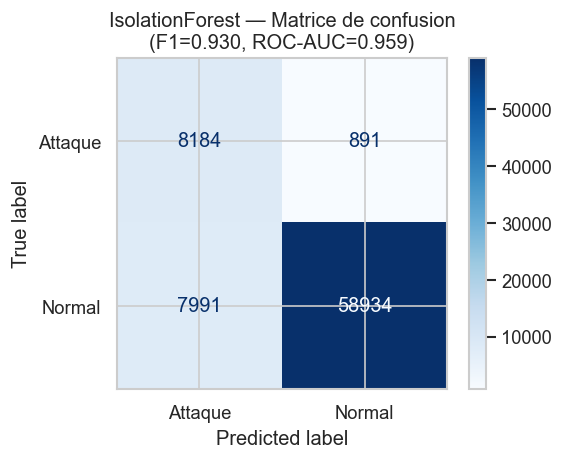
\includegraphics[width=0.6\textwidth]{figures/iso_forest_confusion_matrix.png}
  \caption{Matrice de confusion -- IsolationForest}
  \label{fig:iso_cm}
\end{figure}

\begin{figure}[H]
  \centering
  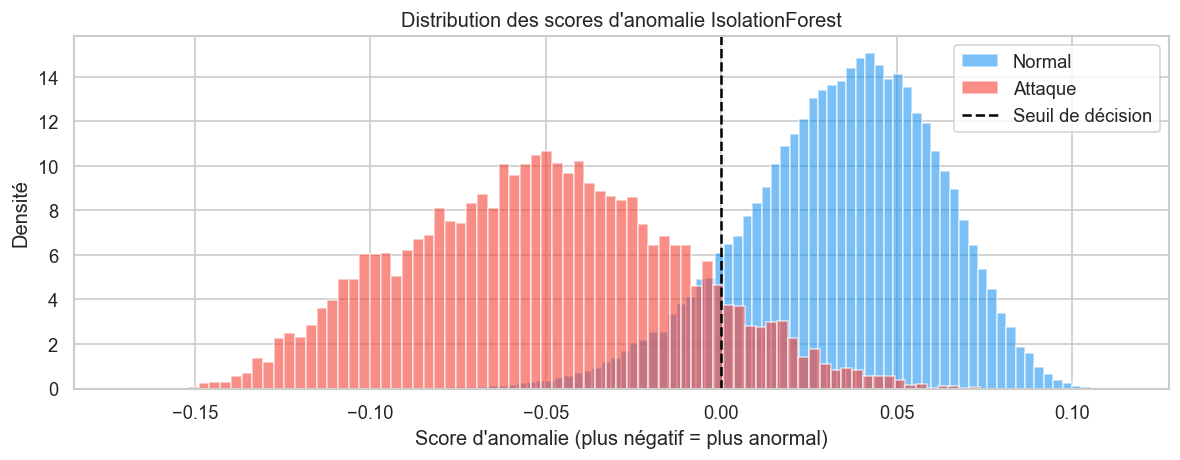
\includegraphics[width=0.7\textwidth]{figures/iso_forest_scores_distribution.png}
  \caption{Distribution des scores d'anomalie -- IsolationForest}
  \label{fig:iso_scores}
\end{figure}

\section{Random Forest -- Détection supervisée}

\subsection{Configuration et entraînement}

Le Random Forest~\cite{breiman2001random} est un ensemble d'arbres de décision entraîné en mode supervisé. Les hyperparamètres sont les suivants :

\begin{table}[H]
\centering
\caption{Hyperparamètres du Random Forest}
\label{tab:rf_params}
\begin{tabular}{ll}
\toprule
\textbf{Paramètre} & \textbf{Valeur} \\
\midrule
\texttt{n\_estimators} & 200 \\
\texttt{max\_depth} & None (pas de limite) \\
\texttt{min\_samples\_split} & 2 \\
\texttt{min\_samples\_leaf} & 1 \\
\texttt{class\_weight} & \texttt{balanced} \\
\texttt{random\_state} & 42 \\
\texttt{n\_jobs} & -1 \\
\bottomrule
\end{tabular}
\end{table}

Le paramètre \texttt{class\_weight='balanced'} est activé pour compenser le déséquilibre des classes du dataset, en attribuant un poids inversement proportionnel à la fréquence de chaque classe.

\subsection{Résultats Random Forest -- Détection binaire}

\begin{table}[H]
\centering
\caption{Métriques Random Forest (détection binaire)}
\label{tab:rf_results}
\begin{tabular}{ll}
\toprule
\textbf{Métrique} & \textbf{Valeur} \\
\midrule
Précision & 0.994 \\
Rappel & 0.993 \\
F1-Score & \textbf{0.994} \\
ROC-AUC & \textbf{0.999} \\
\bottomrule
\end{tabular}
\end{table}

\begin{figure}[H]
  \centering
  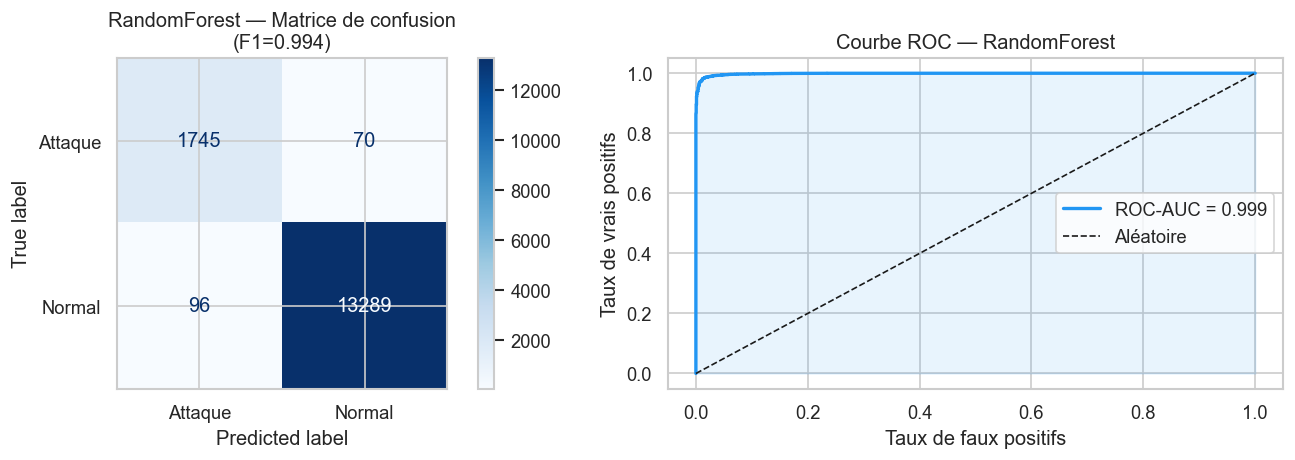
\includegraphics[width=\textwidth]{figures/rf_confusion_roc.png}
  \caption{Matrice de confusion et courbe ROC -- Random Forest}
  \label{fig:rf_roc}
\end{figure}

\begin{figure}[H]
  \centering
  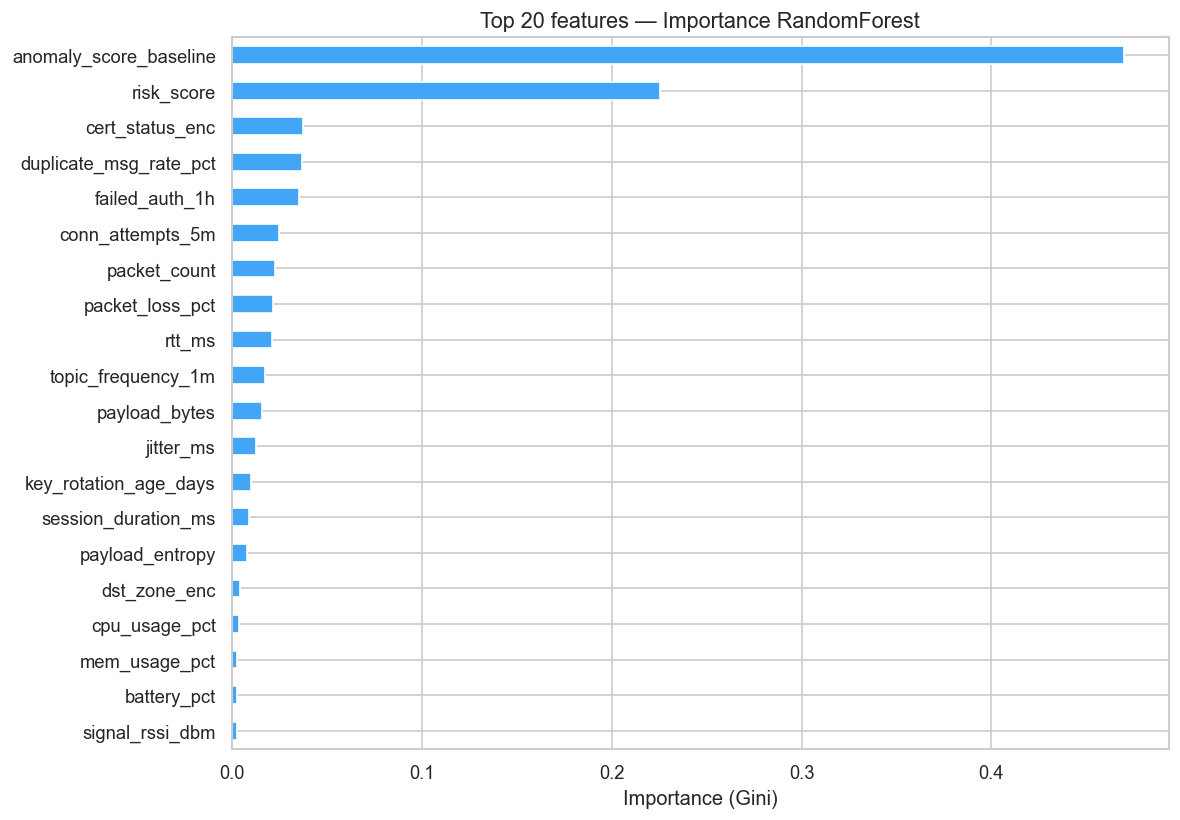
\includegraphics[width=0.8\textwidth]{figures/rf_feature_importance.png}
  \caption{Importance des features -- Random Forest}
  \label{fig:rf_features}
\end{figure}

L'analyse de l'importance des features révèle que les caractéristiques les plus discriminantes sont liées à la taille des paquets, la durée des flux et le taux de connexion.

\subsection{Classification multi-classe}

Un deuxième modèle Random Forest a été entraîné pour la classification multi-classe (7 types d'attaques). Ce modèle atteint un F1-score moyen de \textbf{0,988}, avec des performances légèrement inférieures sur les classes minoritaires (Malware, Scanning).

\begin{figure}[H]
  \centering
  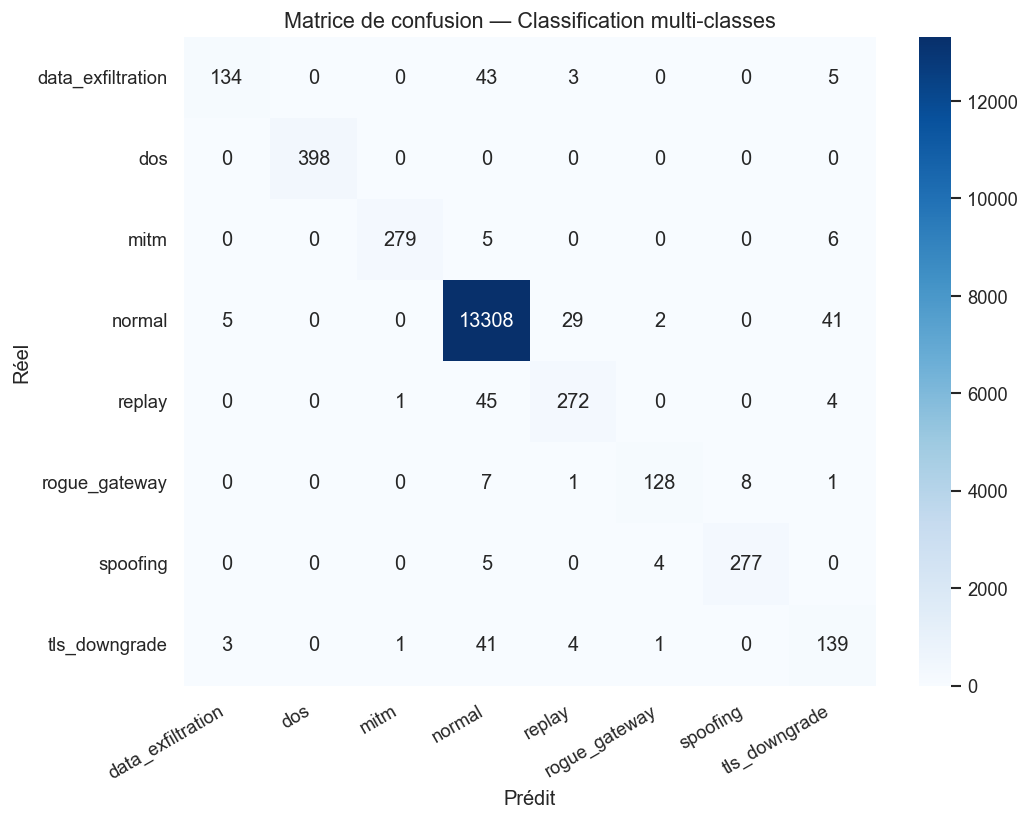
\includegraphics[width=0.8\textwidth]{figures/rf_multiclass_confusion.png}
  \caption{Matrice de confusion multi-classe -- Random Forest}
  \label{fig:rf_multiclass}
\end{figure}

\section{Comparaison des modèles}

\begin{figure}[H]
  \centering
  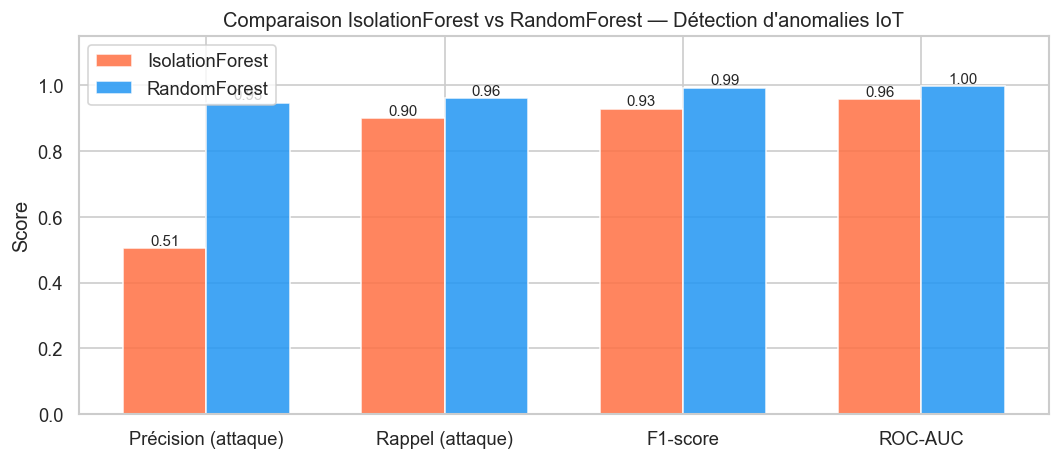
\includegraphics[width=0.8\textwidth]{figures/models_comparison.png}
  \caption{Comparaison IsolationForest vs Random Forest}
  \label{fig:models_comp}
\end{figure}

\begin{table}[H]
\centering
\caption{Comparaison finale des deux approches ML}
\label{tab:ml_comparison}
\begin{tabular}{llll}
\toprule
\textbf{Modèle} & \textbf{F1-Score} & \textbf{ROC-AUC} & \textbf{Type} \\
\midrule
IsolationForest & 0.930 & 0.959 & Non supervisé \\
Random Forest (binaire) & 0.994 & 0.999 & Supervisé \\
Random Forest (multi-classe) & 0.988 & 0.998 & Supervisé \\
\bottomrule
\end{tabular}
\end{table}

\begin{resultbox}[Bilan ML]
Le Random Forest, en mode supervisé, atteint des performances quasi-parfaites (F1=0,994, ROC-AUC=0,999), exploitant les étiquettes pour apprendre les signatures de chaque attaque.

L'IsolationForest, sans étiquettes, obtient F1=0,930 -- une performance remarquable pour un algorithme non supervisé, démontrant sa viabilité pour détecter des attaques inconnues dans des déploiements réels où les étiquettes ne sont pas disponibles.
\end{resultbox}
